\section{Project Description \pagebudget{.5}}

\iflater\todo{Remember to not use any URLs in the project description!
  (They are encouraged in the references.)}\fi

Testing plays a key role in modern software development, contributing
crucially to robustness and overall quality---as well as to overall
development costs.
%
It comes in many styles---unit testing, integration testing,
performance testing, stress testing, accessibility testing,
etc.---supported by many sorts of tools, with yet more advanced tools
and techniques continually being developed, discussed, and applied.
%
One such technique, {\em property-based testing} (PBT), has been
enthusiastically applied and refined within the functional programming
community since its introduction in the Haskell QuickCheck
library~\cite{ClaessenHughes00}.
%
PBT is sometimes explained as ``formal specification without formal
verification''---developers are invited to characterize their program's desired
behaviors at a high level, in the form of executable {\em properties},
which are simply Boolean-valued functions; their code is then validated against
these properties by running it over and over with a large number of
automatically generated test cases.

This combination of rich, high-level specifications with easy, mostly
automatic validation has proved effective at identifying subtle
bugs in telecommunications software~\cite{arts2006testing}, replicated
file~\cite{hughes2014mysteries} and key-value
stores~\cite{Bornholt2021}, car software~\cite{arts2015testing}, and a range
of other real-world systems~\cite{hughes2016experiences}. With tools
now available in all major programming languages, PBT has
begun to make significant inroads in the broader software
industry---for example, the developers of the Hypothesis library for
Python estimate that it has on the order of half a million
users~\cite{ZacPersonalCommunication}.

With all of this success, one might wonder if the research community has already
identified all of the important challenges that limit PBT's adoption, but it
seems that the answer is no.
In an ongoing need-finding study with users of OCaml's QuickCheck testing tool
at Jane Street Capital, a Wall Street financial firm, we have found a healthy
mix of consistent enthusiasm for PBT
% \jsquote{28}{If you’re trying to build something that needs to be
%   reliable and work all the time, [PBT] is worth the
%   investment.\iflater\bcp{This is a paraphrase of what Dani said.  We
%     need to pull the actual quote. }\fi}
% \amh{This quote to me does not convey strong enthusiasm, but
% rather muted pragmatism :-). Maybe another quote would do
% the job better. Or maybe we can include that quote from the
% preliminary study which stated that PBT was 1000x better
% than the alternatives.}
and challenging new research questions based on developer concerns.
Specifically, the developers we have spoken with so far (a) sometimes struggle
to identify all the situations where properties are readily accessible for
testing
% \amh{Here I think it is important to have an affirmation that there
%   are indeed cases where PBT will be valuable to them that they just
%   have not yet identified},
% BCP: Added "all the"--is that enough?
(b) they complain that it
is sometimes difficult to write random generators for data structures
with complex invariants or to tune generator distributions to
adequately explore the space of interesting test cases, (c) they find
it hard to understand whether their properties and generators are
effectively testing their software, and (d) they are disappointed by
the paucity of educational and training materials for introducing
newcomers to PBT.\iflater\bcp{All that needs final tuning.}\fi

The solutions to these problems, much like the techniques that helped us to
identify them, require insights from both the programming languages (PL) and
human-computer interaction (HCI) communities.  Chasins et
al.~\cite{chasins_pl_2021} argue that PL+HCI is a ``sweet spot'' that marries
``need-finding techniques [to] identify ...  programmers' current and future
pain points''
with
``tools that make it easy to build domain-specific and
general-purpose programming languages,''\hg{Try to find a better quote}
and we whole-heartedly agree.

Thus, we propose a comprehensive, interdisciplinary research program that will
bring the power of both PL and HCI techniques to bear: we will build a blueprint
for the future of PBT theory and practice that is motivated by users and built
on solid theoretical results.

\todo{Break this out and bullet it}
Specifically, we aim to (1) further
investigate the challenges PBT faces in industry through
two\iflater\bcp{three?}\fi{}  additional user studies (\sectionref{sec:spec});
address the challenges we have observed in (2) property specification
(\sectionref{sec:spec}), (3) test-case generation
(\sectionref{sec:gen}), and (4) validation of testing effectiveness
(\sectionref{sec:val}) by developing new, theoretically motivated and
rigorously designed, tools; and (5) create comprehensive resources for
educating developers and university students in best practices for PBT
(\sectionref{sec:ed}).
\writeme{Mention broader impacts and work plan sections.}

The projects we undertake will be motivated by
foundational need-finding research in the software industry, including, but not
limited to, the aforementioned study with Jane Street. Some projects will have a
clear PL flavor, focusing on domain-specific languages and type-based tools that
will make PBT tools more powerful and flexible; but we will motivate and
evaluate them with techniques from HCI. Other projects will focus on the HCI elements
of PBT, building better interfaces and experiences for developers; yet their
implementation will draw from our wealth of PL knowledge. In this way, we craft
a holistic research agenda around PBT that is sure to be both well motivated and
well founded.

% Testing plays a central role in modern software development,
% contributing crucially both to the costs of software projects and to
% the quality of their results.
% %
% Testing comes in many styles---unit testing, integration testing,
% performance testing, stress testing, accessibility testing,
% etc.---supported by many sorts of tools, with yet more advanced tools
% and techniques continually being developed, discussed, and applied.

% One such technique, {\em property-based testing} (PBT), has enjoyed
% widespread popularity in the functional programming community since
% its introduction in the QuickCheck library~\cite{ClaessenHughes00} in
% Haskell.  PBT can be thought of as a kind of ``formal specification
% without formal verification.''  Programmers are invited to
% characterize the desired behaviors of their software systems or
% individual components at a high level, in the form of abstract models
% or algebraic laws; their code is then validated against these
% specifications by running it against a large number of automatically
% generated test cases.

% This combination of rich, high-level specifications with easy, mostly
% automatic validation has proved extremely effective at flushing out
% bugs in telecommunications software~\cite{arts2006testing}, replicated
% file~\cite{hughes2014mysteries} and key-value
% stores~\cite{Bornholt2021}, cars~\cite{arts2015testing}, and a range
% of other real-world systems~\cite{hughes2016experiences}.  With PBT
% tools now available in pretty much every major programming language,
% PBT has begun to make significant inroads in the broader software
% industry---for example, the developers of the Hypothesis library for
% Python estimate that it has on the order of half a million
% users~\cite{ZacPersonalCommunication}---creating large benefits in
% productivity and software quality for its users.\iflater\bcp{Can we
%   justify that?}\fi

% What would it take to make the benefits of PBT available to an even
% broader community of software developers?  Maybe not so much.

% In an ongoing study of users of OCaml's QuickCheck testing tool at
% Jane Street Capital, a Wall Street financial firm, we have heard
% strong enthusiasm tempered by a degree of frustration on a few fronts.
% These users generally appreciate PBT for its power and broad
% applicability, but (a) they sometimes struggle to identify
% situations where PBT will be valuable,
% (b) they complain that it
% is sometimes difficult to write random generators for data structures
% with complex invariants or to tune generator distributions tg
% adequately explore the space of interesting test cases, (c) they find
% it hard to understand whether their properties and generators are
% effectively testing their software, and (d) they are disappointed by
% the paucity of educational and training materials for introducing
% newcomers to PBT.  \iflater\bcp{All that needs final tuning.}\fi
% %
% Fortunately, we believe all these difficulties can be significantly
% improved with a modest amount of suitably focused research energy.  We
% propose to provide it.

% The remainder of this section introduces property-based testing and
% describes the findings of the Jane Street user study in more detail,
% to motivate and contextualize the work planned for this project.  The
% remaining sections describe several threads of planned work and their
% expected contributions.  Specifically, we aim to (1) further
% investigate the challenges PBT faces in industry through
% two\bcp{three?}  additional user studies (\sectionref{sec:spec});
% address the challenges we have observed in (2) property specification
% (\sectionref{sec:spec}), (3) test-case generation
% (\sectionref{sec:gen}), and (4) validation of testing effectiveness
% (\sectionref{sec:val}) by developing new, theoretically motivated and
% rigorously designed, tools; and (5) create comprehensive resources for
% educating developers and university students in best practices for PBT
% (\sectionref{sec:ed}).  \bcp{This is OK as a TOC, but as an
%   advertisement of planned contributions it is still pretty
%   lacking. We'll need to either add a separate contributions paragraph
%   someplace later or (better, I think) beef up this one.}
% \bcp{Need to mention broader impacts and work plan sections.}


\subsectionstar{Orientation: Property-Based Testing}
\bcp{Added this sentence per Andrew, but I wonder if it belongs earlier}
Property-based testing tools give programmers
an efficient way of testing their software's behavior with a
comprehensiveness that is often not possible with alternative tools.

PBT tools allow users to write executable functions
that act as partial
specifications of a function under test. For example, a user might
write the following property of the \lstinline{insert}
function for an implementation of a binary search tree (BST):
\begin{lstlisting}
  prop_insertCorrect x t  =  (isBST t ==> isBST (insert x t))
\end{lstlisting}
This property takes only a single
line to express, yet it can be used to validate a limitless number of
input-output pairs. Concretely, it is
a simple function that takes two arguments and returns a
Boolean value: true if the property is satisfied, and false if it is
not. The function \texttt{prop\_insertCorrect} checks
that an insert operation on a binary search tree preserves the
binary ordering of the tree; it states
that, given an arbitrary tree \texttt{t} and an integer
\texttt{x} to insert into that tree, if the original tree
satisfies the
binary search tree invariant (``\texttt{isBST t}''), then it should remain
a BST following the insertion of \texttt{x} (``\texttt{isBST (insert x t)})''.

\iflater \bcp{I think this point will show up later:}There are a
myriad of different kinds of properties that one might use to specify
a system; a good source of examples is \citet{HowToSpecifyIt}.  \fi

Given a property like this one, the PBT tool generates a large number of inputs and
checks that the property evaluates to \lstinline{True} for each input.
Any input that causes the property to fail is reported as a {\em
counterexample}. If no counterexample is found after many test
inputs are tried, a developer is given more confidence that their implementation
of the function is correct, given that the properties hold for many
tested configurations.

% \amh{[small change] I removed ``Our focus'' because it felt like it
% was leading towards a statement of our contributions, which I want
% to discourage a reader from thinking we're trying to talk about
% in this background section.}
% BCP: Even better is to move this whole discussion to later -- I've
% done so.  :-)

One well-known challenge of random testing is that some work is often
required to generate {\em well-distributed} random inputs, which can
have a large effect on testing effectiveness; to achieve good testing,
programmers are thus often forced to tune these distribution
manually~\cite{DBLP:conf/icfp/ClaessenH00}. Even more importantly,
testers need to ensure that the sampled inputs are {\em valid} to test
with; we address these issues in \sectionref{sec:gen}.

\bcp{Related work to mention: HypoFuzz \url{https://hypofuzz.com}}
\bcp{This is probably the place to mention a whole ton of related
  work, no?}

\bcp{This is also the place to make our strongest argument for
  potential impact: Why is PBT so much better than standard unit and
  integration testing (at least sometimes)---e.g., its thoroughness,
  ability to discover weird edge cases, value as documentation, ease
  of application (in some common cases), ... what else?} \amh{+1}

\amh{[content request] I also think it would be useful to briefly spell out the programming
tasks related to PBT. What do programmers have to write code for to make
PBT work? (1) They need to define a property (one was given above);
(2) They need to define a generator (this is only implied by the above),
which can be done by either writing a program that generates inputs,
or by using tools that infer generators based on type definitions; (3)
They need to write some test driver code that looks for the properties
and generators and executes them. And then, (4) a programmer has to
make sense of the output of the generators and counterexamples, perhaps
by inspecting console logs\ldots{} I think it is important to foreshadow
in this section the different points in the engineering process
where tools can be created, because I think it will be clunky to try to
introduce them alongside novel findings in the ``Motivation'' or ``Foundations'' sections.}\bcp{Yes!!}

\subsectionstar{Motivation: A Formative Study of PBT in Industry \pagebudget{2}}\label{sec:motivation}

\iflater\todo{Fix the capitalization.  :-(}\fi

\todo{
  \begin{itemize}
    \item MOTIVATION SECTION
    \begin{itemize}
      \item Motivating questions for JS study
      \item Lay out study parameters in some (but not much) detail
      \item Discuss some emerging themes
      \begin{itemize}
        \item Give justification in the form of quotes for some
        \item Say why the themes are important, how they line up with existing
        understanding
        \item Situate themes relative to their categories
      \end{itemize}
      \item Tie everything together
      \begin{itemize}
        \item The themes of this study map onto the projects that we plan to
        carry out
        \item Each theme category has a section below, each project in those
        sections directly serves one or more of the themes in that category
        \item Here's what we're going to do...
      \end{itemize}
    \end{itemize}
  \end{itemize}
}

\hg{Pulled from the section below, we'll need to massage}
The first step is to conduct qualitative interviews to understand the challenges
that programmers face when using PBT tools. To this end, we plan to undertake an
interview study with our research partner, Jane Street, LLC\footnote{See letter
of support in the appendix.} to develop a deep understanding of the challenges
programmers face using PBT in industrial settings as well as being to explore
potential solutions.

TODO: Jane Street Capital is one of the world's largest market-makers,
with over 1700 employees including around 700 software developers...

\textbf{Research questions}.
Our key research question will be, \emph{How can the research community make PBT
more valuable for software developers?} More specifically, we seek
answers to the following questions:

\begin{itemize}[noitemsep,leftmargin=4em]
\item[\bf RQ1.] What support do developers need to help them imagine properties? \todo{Reword, the notion of ``imagining'' properties has not yet been introduced.}
\item[\bf RQ2.] What kinds of generators do testers need to exercise their
  properties effectively? Do they have specific precondition and/or distributional
  requirements?
\item[\bf RQ3.] What aspects of the developer workflow around PBT need improvement?
\item[\bf RQ4.] What concrete changes could be made to modern PBT systems
  to improve effectiveness and usability?
\end{itemize}

{\bf RQ1}, {\bf RQ2}, and {\bf RQ3} relate to property,
generator, and workflow challenges, respectively.
{\bf RQ4} more directly asks how existing systems might
be improved. This final question will help to keep us focused,
reminding us that participants likely have the context and knowledge not
only to identify challenges but also to suggest
solutions.

\textbf{Research site}. We will partner with Jane Street, LLC, a large
financial technology firm.
Jane Street has a number of qualities that makes it an ideal place for
this study. To start, Jane Street developers use
a variety of testing tools, including PBT. This gives us a place to start
when asking questions, since participants will likely have seen PBT before,
and it means that will be score for exploring trade-offs between PBT and
other forms of testing.
Additionally, Jane Street developers famously build almost all of their
systems in OCaml, a mostly functional programming language with strong support
for static typing and modularity. This unified ecosystem
will allow
us to control for a number of potentially confounding factors: all of the
developers we talk to will have access to the same PBT tools and the same
libraries, language-level programming abstractions, house coding rules,
etc. (which might make testing easier or harder).

Naturally, carrying out a study at a single firm has potential drawbacks as
well. The most obvious is that our results may not generalize: We
cannot guarantee that our findings will apply outside of the OCaml ecosystem (and
other ecosystems like it). However, Jane Street is home to a diverse array of
software systems, including trading systems, quantitative
algorithms, networked systems, and hardware description code~\cite{signalsandthreads}.
We hope that the breadth of these programming tasks will mean that the software
developers that we talk to will come to the discussion with a wide variety of
experiences.


\subsectionstar{Personnel}

\todo{One paragraph about what a great team we are, how the PI
  qualifications complement each other, and what kind of students we
  aim to support.}

% We have seen these trends firsthand: the PL research group at Penn has
% contributed to PBT research for years, pushing PBT to its limits as a
% tool for standard
% testing software~\cite{hughes2014mysteries, li_model-based_2021,
% goldstein2021dojudgeatest, goldstein2022parsing} and adapting it to new domains
% like theorem proving~\cite{paraskevopoulou_foundational_2015,
% lampropoulos_coverage_2019}.  The community has dedicated itself to improving
% the theory and applications of PBT, and recent work has continued to make great
% strides in areas like expressivity and testing effectiveness.


\subsection{Foundation: Understanding Needs and Opportunities \pagebudget{1}}

As PBT sees wider adoption, new opportunities present for understanding how
these tools are being used in practice, and how these tools can be further
developed to better support developers' needs. In this section, we describe a
sequence of studies we will undertake to better understand developers' needs.
These studies will draw on mixed methods in the service of producing a
comprehensive and actionable agenda for future research.  Phases of this
research include interviews to develop an initial taxonomy of needs and
obstacles to tool use (Section~\ref{sec:interviews}), a survey to assess the
generality of these needs and obstacles and to identify potential for adoption
of PBT tools (Section~\ref{sec:survey}), and observations to understand
particular tasks involved in PBT to an extent that we can understand how to
design new algorithms and interactive tools that better support those tasks
(Section~\ref{sec:observations}).

\subsubsection{Ongoing Work: Need-Finding Interviews with Jane Street}
\label{sec:interviews}

We will begin our need-finding work by interviewing developers who can shed
light into how PBT is already being used, and obstacles in its use. Interview
studies are common in early-stage need-finding research, due to their ability
to yield highly informative stories about people, the tasks they need to
accomplish, and the tools they use to accomplish them. The purpose of these
interviews is to identify a broad set of opportunities for improving PBT tools,
grounded in concrete, authentic, detailed stories from developers.

\textbf{Method}. Semistructured interviews will be conducted with approximately
30 developers. Questions will focus on tasks these developers wish to accomplish
with PBT tools, and around developers' recollections of what it was like to
work with PBT tools to accomplish these tasks.

\textbf{Population}. Ideally, these interviews would involve both current users
of PBT as well as non-users of PBT. In reality, it is difficult to recruit and
have meaningful conversations with non-users of a technology. We plan to
recruit users across as broad a spectrum of usage as we can reasonably recruit,
including both frequent users of PBT technologies, as well as a handful of
developers who have had only limited, occasional exposure to PBT. Our survey
study (Section~\ref{sec:survey}) aims to establish contact with a broader
sample of non-users of PBT to assess opportunities for making PBT tools more
valuable and discoverable for this group.

\textbf{Progress}. Our interview instrument and analysis process was developed
and tested with 7 users of the Hypothesis PBT toolkit, recruited over Twitter.
This analysis yielded a conceptual framework of barriers to usage of PBT, which
we published recently at HATRA, an ACM SPLASH workshop and one of the key
venues for presenting preliminary research on human aspects of formal methods
tools and type systems~\cite{goldstein2022some}.

We have since established a collaboration with Jane Street, LLC\footnote{See
the attached letter of support.} with whom we will conduct an expanded
interview study. To date, through this collaboration we have already conducted
27 of 30 interviews, including both developers who have had exposure to PBT as
well as developers of PBT tools. Our interview process has included an on-site
visit where we collected feedback on our evolving conceptual framework of the
needs and opportunities we have discerned around PBT tools.

What remains for this project is another approximately 2 months of Ph.D.
student work, including conducting the remaining interviews, performing
in-depth qualitative analysis of the data following a thematic analysis
approach~\cite[Chapter 5]{blandford2016qualitative}, and preparing a manuscript
for submission to OOPSLA.

\textbf{Preliminary results}. Key takeaways emerging from our initial analysis
appear in Section~\ref{sec:motivation}.\amh{Is there anything else we want to
say here about the results?} \amh{Let's recapitulate the major findings that
motivate this proposal as a whole. Then, let's foreshadow other findings that
we will publish that are outside of the scope of this proposal, but which might
be motivating to other researchers, including: developers could benefit from
additional automated support for deriving generators from types, effectiveness
budget (i.e., deciding how much time to spend on running PBT tests versus fuzz
tests), integration with unit testing frameworks, and exploring the use of
properties as a source of documentation.}

\subsubsection{Proposed Work: Surveys to generalize findings}
\label{sec:survey}

% \subsubsection{Proposed Work: Characterizing the Potential for Impact in Improved PBT Tools}

Our interview study will reveal a number of opportunities to
improve tools for property-based testing. To help us
validate the conclusions from the interviews, and to help us
identify the potential of this project as a whole for
meaningfully impacting the work of developers, we will
conduct two surveys with broad populations of developers.

\emph{Validation survey}. What usability issues from the
usability study most merit additional attention from the
research community? To answer this question, we will conduct
a validation survey with current users of PBT tools.
\amh{Continue from here. Mention that this survey will be
conducted with users of a variety of a set of PBT tools. The
purpose of the survey will be to both assess the frequency
with which certain kinds of usability issues arise, as well
as the severity of those issues.}

\emph{Impact survey}. As evidenced in this proposal through
the usage stories we have shared from the research
literature and interviews, PBT has been demonstrated to have
massive potential for helping individual developers validate
their software. That said, what is less clear is the breadth
of applicability of these technologies. Is PBT the sort of
technology that one day would be used by every developer? Or
instead by the set of developers who use it today? We
anticipate it is somewhere in between. To help the research
field as a whole assess the potential impact of developments
in PBT technology, we will conduct a survey to attain better
estimates of the group of proximal users of PBT---that is,
those users who do not use PBT currently, but who experience
use cases where PBT methods would be particularly useful,
once designed to fit their tasks and workflows. Particular
attention will be given to those whose work requires the
writing of validation code and public APIs with some
definition of types. We will recruit a broad sample of
participants across development contexts (professional, open
source, educational) by working with our industry contact
and by recruiting over social media. \amh{I am not sure this
survey feels quite right. It feels really hard to conduct in
a way that we get a convincing answer to our question of
``who would use PBT if the tools were sufficiently
well-designed?''}

\amh{Mention that we plan to distribute a survey among users of Hypothesis to
assess the extent to which our findings generalize among a broader population of
users of PBT tools. Can we get a letter of support from Zac?}\bcp{We should!!}

\amh{I think we need to conduct two studies, one focused on assessing the
extent to which our findings about obstacles generalize across PBT users
broadly, and one assessing the extent of potential adoption of these tools,
if major obstacles to adoption are lowered.}

\subsubsection{Proposed Work: Observations of PBT in practice}
\label{sec:observations}

\amh{The areas where I think we could most benefit from better understanding
PBT tasks in detail are (1) generator design, implementation, and evaluation;
(2) evaluating the results of properties (in particular, debugging and addressing
counterexamples). I think that our success in designing appropriate tools for
developers might depend on us having a clearer understanding of what it looks
like for developers to undertake these tasks.}

The next step is to more deeply characterize the obstacles faced with specific
tools and tasks through close observation. We anticipate conducting observations
of participants formulating properties and creating generators, as we expect
that close observation of developers performing these tasks will yield yet
additional detail about ways that developers are supported and not supported by
the tools they use today to a level of depth we will not achieve with the
interviews.

\subsection{Step 1, Specification: Widening the On-Ramp to Properties \pagebudget{2}}\label{sec:spec}
\subsubsection{Proposed Work: When to Specify It!}
Since PBT is often described as a kind of lightweight formal method, one might
have imagined that a central challenge of using PBT would be coming up with the
right specifications. Indeed, our preliminary study concluded just that. But at
Jane Street we actually heard very little about the challenge of coming up with
properties; instead, most participants described applying PBT in scenarios when
properties were already available or quite easy to imagine. This suggests that,
while PBT education should certainly spend some time teaching developers how to
write specifications for arbitrary programs, it should spend even more energy
helping developers quickly recognize  situations where PBT is a particularly
natural fit because properties are obvious.

With this in mind, we plan to write a short paper (with an accompanying talk)
entitled {\em When to Specify It!}. The paper will be a spiritual successor to
John Hughes's {\em How to Specify It!}~\cite{HowToSpecifyIt}, a lovely account
of the many different kinds of properties that one can write for a given piece
of code. Clearly it is important to ask {\em How}, but the developer interviews
suggest that it may be even more important to have a clear sense of {\em When}
to use PBT. {\em When to Specify It!} will combine examples from developer
interviews with ones from our our years of experience studying and applying PBT
into the definitive guide for the most impactful opportunities to apply PBT.
\hg{Do we need more here? I can give examples...}
% \begin{itemize}
% \item Code that is already (semi-)formally specified.
% \item Functions that round trip.
% \item Pure data structures.
% \item Modules with invariants.
% \item Related versions of the same code.
% \item Programs that may fail catastrophically.
% \item Stateful APIs with well-understood contracts.
% \end{itemize}

\subsubsection{Proposed Work: Properties Over Logged Output}
One common problem raised by Jane Street developers (and even more loudly by the
participants of the \hg{preliminary}) study was that code may not be abstracted
in a way that is conducive to PBT. Indeed, any kind of unit testing requires
that the programmer is able to extract some ``unit'' of code to test, but PBT is
especially sensitive to things like poorly handled global state and fuzzy
abstraction boundaries. Fuzzers \todo{I think we need to intro fuzzers in the
beginning; I've mentioned them a bunch already} get around these issues by
testing the code from the outside---they do not care about internal
abstractions, only the external interface---but that usually comes at the
expense of expressive properties.

We hypothesize a solution that enables better PBT of messy code without giving
up expressiveness: inject logging calls into the code under test, and write
properties over the logs that the code produces. For example, if the developer
knows about some invariant on a variable \lstinline{x}, they can log out the
value of \lstinline{x} every time it is set, and then check that the logged
values satisfy the invariant. Even better, if the invariant applies over time
(e.g., the value of \lstinline{x} should never decrease) properties over logs
could capture that too. This would be difficult to do with debug assertions,
especially if performance is a concern.

Concretely, we propose a framework for inserting lightweight test-logging and a
language for writing properties over those logs. The logging itself is a matter
of engineering, but the language for properties is an exciting opportunity to
apply powerful logical ideas. Specifically, the properties over logged outputs
should be written in a temporal logic like {\em linear temporal logic} (LTL) so
they can make complex assertions about the way past and future values interact.
The Quickstrom language~\cite{oconnor_quickstrom_2022} has already shown that
LTL properties are possible (it uses LTL to write properties about graphical
user interfaces), but making them work well for a broader range of scenarios is
an exciting research challenge.

\subsubsection{Proposed Work: Automating Model-Based PBT}
Our studies have shown that a common pattern of PBT, especially for stateful
APIs, is to implement a {\em model implementation} of the system under test, and
then check that the two versions of the code agree on a series of API calls.
This is a well documented approach to PBT~\cite{hughes_experiences_2016}, but it
is not always supported as well as it could be by existing tooling. For example,
developers at Jane Street cited setting up essentially the same basic
model-based PBT harness for at least three different projects; implementing each
of those harnesses took significant developer time and slowed down the testing
process.

We propose new, type-based automation for model-based testing of ML-style
modules. This automation will take a model signature, for example
\begin{lstlisting}[language=Caml]
  module Map : sig
    type ('k, 'v) t
    val get : ('k, 'v) t -> 'k -> 'v option
    val put : ('k, 'v) t -> 'k -> 'v -> ('k, 'v) t
  end
\end{lstlisting}
and generate a series of calls like
\begin{lstlisting}[language=Caml]
  let m = put m 1 2; get m 1; let m = put m 1 3; m get 1
\end{lstlisting}
that manipulate the data structure and query its contents. When testing two
different implementations of \lstinline{Map}, the developer can verify that the
two implementations produce the same results for each of the operations in the
sequence. The automated tooling could also insert checks for internal
invariants, ensure that one operation executes at least as quickly as another,
and insert other checks that are simple to specify but tedious to implement
manually.

Our choice to focus on ML-style modules is motivated from two directions. One is
practical: our relationship with Jane Street makes it easy to evaluate tools
that are compatible with OCaml, the language that almost all of their developers
are the most comfortable with. Working within the OCaml ecosystem will mean that
we can quickly find technical or usability issues with the tools we build. The
other reason, though, is technical interest. ML modules are extremely
expressive and fairly complicated. This gives us a number of complex problems to
solve: for example, \todo{Maybe have Joe look at this section. He really likes
this project}

\subsubsection{Proposed Work: Interactive Property Specification}

\bcp{General comment for this section: It all seems good, but it is a bit vague
and high level---I feel like technical readers will want a bit more meat.  Could
we spice it up with a concrete example?  (Indeed, should we be thinking about a
running example for the whole proposal?)} \amh{Agreed, I think a concrete
example would be \emph{great} here. Maybe there is an example we can bring in
from the QuickSpec paper~\cite{claessen2010quickspec}}

As our preliminary interview study has suggested, developers sometimes have
difficulty imagining which properties to test, even when they know that their
software would benefit from property-based testing. One area we are interested
in exploring is how programmers can work with their PBT tools to decide on a set
of significant properties to test.  Prior research demonstrates that automated
tools can extract specifications of a program's
behavior\cite{ammons2002mining,le2018deep,claessen2010quickspec}. We are
interested in the non-trivial research problem of integrating such techniques
into usable developer tools. We see the research as addressing several
challenges:

\textit{Generated properties should be \emph{important}}. Any non-trivial
program can be characterized by an overwhelmingly large number of properties,
many of which describe only incidental aspects of the program's behavior that do
not need to be tested. How can tools produce those properties that developers
would want to have tested? We believe that this is a problem that can be best
solved with a mixed-initiative approach~\cite{allen1999mixed}, where properties
are determined by judiciously incorporating both developer input and automated
techniques.

Developer could guide a specification mining tool to extracting relevant
properties through input mechanisms such as (1) identifying regions of code that
are likely to lead to an adverse behavior such as an exception or a logical
error; (2) providing unit test cases that test a special case of a generalized
property; and (3) indicating aspects of interest on input and output data during
exploration in a debugging REPL.

\textit{Generated properties should be \emph{readable}}. While prior research
has shown promise for automatically generating specifications of program
behavior, we expect that users of PBT systems would benefit from having
properties generated in the language of their property-based testing tools.
Furthermore, there are some variants about systems that may be so complex that
they require significant comprehension time for users (i.e., those involving a
large number of clauses). In such cases, a tool may way to generate simpler
variants of properties first, and allow developers to refine them on their own.

\textit{Tools should help developers \emph{revise} properties}. If a generated
property is too relaxed, the tool should request that developer provides a
counterexample that should trigger a failure, and then regenerate the property.
If a generated property is too strict, a tool should allow a programmer to mark
a counterexample that was generated by the PBT tool as spurious, i.e., not
indicating an actual failure of the program. In each of these cases, the
property generator may have generate multiple properties for a developer to
review, each of which may satisfy the refinements that a developer has provided.

\textit{Plan of work}: We will iteratively design and develop developer tools as
an extension to the VSCode editor, a popular development environment for
Haskell. In our first iterations, candidate properties will be generated using
QuickSpec~\cite{claessen2010quickspec}. The interactions described above will be
designed and tested first for simple programs, and then on successively more
complex programs from our benchmark set. PI Head has extensive experience
designing and developing developer tools involving program
analysis~\cite{head2018interactive,head2019managing} and program
synthesis~\cite{head2017writing} components, and extending the VSCode
environment~\cite{head2020composing}.  \bcp{Maybe consider focusing on OCaml
tools, rather than Haskell, since this is where there might be synergy with Jane
Street?  Or do both?} \amh{This is a great idea. Does anyone know of any
specification generators for OCaml?}

\subsection{Step 2, Generation: Better Tools for Random Inputs \pagebudget{3}}\label{sec:gen}
\hg{Half page over at the moment}\bcp{Made it a bit worse by moving
  the discussion of random vs. enumerative here... :-)}

\bcp{The opening needs tuning.}
Our focus in this proposal is on {\em random}
testing~\cite{hamlet1994random}, where the inputs used to validate a
property are generated by some random process, but there are other
alternatives. In particular, {\em enumerative
  testing}~\cite[etc.]{DBLP:conf/haskell/RuncimanNL08, leancheck}
deterministically lists every possible input from the smallest to the
largest, and its effectiveness relies on the ``small scope
hypothesis''~\cite{jackson1996elements} that most bugs can be found
with ``small'' inputs. Some\iflater\bcp{which?}\fi{} forms of model
checking can also be considered alternatives to random PBT; their
approaches vary, but, to a first approximation, model checkers are
essentially tools for searching an input space for
counterexamples~\cite{biere2009bounded}.
%
Despite the success of enumerative test-case generation and model
checking, random generation remains the dominant approach in the PBT
space. Its surprising effectiveness is often attributed to the
``combinatorial'' nature of larger test cases: bugs can often be
exposed by test inputs with a specific combination of features,
independent of whatever other features may be present---for example,
by any sequence of API calls that includes calls to four particular
functions in a particular order, even if these calls happens to be
interleaved with other API calls.  This means that testing with one
big structure has the effect of testing with exponentially many
smaller sub-structures. Both practical experience and theoretical
arguments~\cite{HarryPaper} suggest that this effect is quite
powerful---i.e., we can discover small counterexamples by generating
a few larger test inputs containing combinatorially many diverse
sub-structures rather than systematically enumerating test inputs
beginning with the smallest ones. \amh{[shorten] We can probably shorten the
above paragraph---I am not sure that we need to sell random testing as
a paradigm, given that it seems the dominant form of testing in PBT
tools today. The detailed comparison to enumerative testing feels
a bit distracting to me. I think it's enough to say that we would
just want to better support random testing because it is the approach
that people are already using.}

\bcp{Work needed here on the transition.}

One of the most important, and most and difficult, tasks in the PBT process is
designing and implementing the random data generators that are used check that
each property holds. Indeed, recall that developers we interviewed consistently
cited designing generators one of the hardest parts of the PBT process, and many
developers asked for better tools for constructing generators that accomplish
their testing goals. In this section, we discuss a series of projects that build
on a rich literature to develop new and better ways to express random data
generators.

\subsubsectionstar{Context: Why is input selection hard?}%
Before presenting our proposed work to improve the state of random data
generators, we must first discuss the major difficulties with random generation
for PBT and the existing work that aims to address those difficulties.
\todo{Link all of this to the intro}

\todo{Talk about enumeration}

{\em Preconditions.}
Many properties that developers want to test have {\em preconditions}
(equivalently {\em validity conditions} or {\em input constraints}) that
restrict the set of inputs that should be used for testing. This comes up often
when testing data structures with invariants that must hold in order to apply
the operations under test. Testing such properties can be problematic, because
many preconditions are difficult to satisfy randomly; if the developer is not
careful they may waste considerable time generating and discarding invalid inputs.

{\em Coverage of Realistic Inputs.}
Even among valid inputs, not all are equally realistic. Often generated inputs
feel fabricated, since they are not constructed with prior knowledge of the
kinds of inputs that the program is likely to see.

{\em Other Distributional Concerns.}
And {\em even} with validity and realism accounted for, there are other ways for
generators to under-perform. In particular, the spaces of inputs that generators
target is often very large, and the best generators explore the whole space as
quickly as possible. This often (but not always) leads users to manually tune
the weights on generators' choices to ensure that the generator does not spend
too much time in one part of the space or another.

\todo{Make sure we tailor the explanations above to the problems we actually
solve, and then make it clear when we've solved one of the problems.}

The literature addresses these concerns to various degrees, and existing tools
fall on a spectrum from automatic to manual. The automatic approaches use
proxies for validity and general ``interestingness'' of inputs: some optimize
readily available metrics like code coverage~\cite{afl-readme}, others ask users
to provide metics~\cite{loscher2017targetedpbt}, and, naturally, a few use
machine learning to infer proxies for validity~\cite{godefroid2017learn,
DBLP:conf/icse/ReddyLPS20}. Slightly more manual approaches are based on
declarative representations of validity conditions: for preconditions that are
primarily structural, {\em grammar-based fuzzing} provides a compelling
solution~\cite{godefroid2008grammar, holler2012fuzzing, veggalam2016ifuzzer,
wang2019superion, srivastava2021gramatron}, and for more complex, semantic
preconditions, some have proposed using SMT-solvers
programming~\cite{dewey2017automated, LuckPOPL, steinhofel2022input} to
automatically seek out valid inputs. This semi-automatic category also includes
tools for {\em example-based tuning}, a process that improves realism of inputs
by mimicking user-provided examples~\cite{soremekun2020inputs}.

The most manual, but also the most flexible, solutions use hand-written
generators, written in a convenient domain-specific language. These are the
topic of the next section.

\subsubsectionstar{Context: Monadic Generators}
When writing generators manually, it helps to have a clean domain-specific
language (DSL) for writing them down. In the Haskell language, where PBT was
first popularized, many such DSLs are implemented using {\em
monads\/}~\cite{moggi1991notions}, which are an elegant design pattern for
expressing effectful (in this case, random and stateful) computations in a pure
language. While monadic DSLs are not actually necessary to express generators in
non-pure languages, some libraries (e.g., in OCaml) still use monadic
abstractions to build their generator DSLs.

Monadic generators implement random data producers of arbitrary complexity
(e.g., it is possible to write a monadic generator for well-typed System F
terms), so they are often more expressive than other representations like
grammar-based generators.  Yet, monadic generators are syntactically constrained
in a way that isolates the probabilistic code and prevents usage errors (like
passing the wrong random seed around). As we will see, the constrained nature of
monadic generators also makes them the perfect candidates for sophisticated
manipulations and interesting generalizations.

\subsubsection{Prior Work: Free Generators}
In order to improve monadic generation along the dimensions listed above, we
choose to re-frame generators as {\em parsers of randomness}. A generator
operates by making a series of random choices, but we can equivalently think of
it as being provided some random sequence of choices and then simply following
those choices to produce a value. This perspective has been used in a few
implementations of PBT systems~\cite{maciver2019hypothesis,dolan2017testing},
but we made it formal in our paper, {\em Parsing
Randomness}~\cite{goldstein2022parsing}.

The paper introduces {\em free generators}, which generalize the standard
monadic generator abstraction, demonstrate a formal link between parsing and
random generation, and enable new algorithms for generation that improve
generation modulo validity constraints. Free generators are written the same
way as standard monadic generators, but they are more like generator ``plans''
or syntax trees.%
\footnote{Free generators are implemented using {\em freer
monads}~\cite{kiselyov2015freer}, which have been used to great effect in recent
years to capture the structure of effectful computations
(cf.~ITrees~\cite{old:xia2019interaction}). Freer monads represent
monadic computations syntactically by reifying the monad operations
(\lstinline{return} and \lstinline{>>=}) as data constructors. Critically, this
is all implemented within the language (no macros or AST manipulation). See the
paper for more details on the free generator representation.}
This means that a single free generator can be be {\em interpreted} in multiple
different ways. In {\em Parsing Randomness} we prove that any free generator can
be interpreted either as a standard monadic generator or as a source of
random choice strings with a parser over those strings; this formalizes the
relationship between generators and parsers. Furthermore, since free generators
are uninterpreted syntax trees, they can be manipulated programmatically. Free
generators admit a version of a Brzozowski
derivative~\cite{brzozowski1964derivatives} that can be used incrementalize
generation. We show that free generator derivatives enable an algorithm called
{\em Choice Gradient Sampling}, which uses repeated derivatives to guide a
generator to inputs that are more likely to be valid with respect to a given
precondition. This work is an important step towards better automation for
generators with complex preconditions.

\subsubsection{Ongoing Work: Reflective Generators}
Continuing on from the free generator work, we have begun to look at even more
powerful generalizations of the standard monadic approach to random generation.
One such project, which is already well underway, concerns monadic generators
that can be run {\em backward}.

If a generator parses a sequence of choices into a value, then running the
generator backward should take a value and produce a sequence of choices that
would produce that value. With this in mind, we present {\em reflective
generators}, an extension of monadic generators that can be run backward to
``reflect'' on the choices that they made when producing an input. The machinery
that makes reflective generators work is quite complex,%
\footnote{Reflective generators are both monads and {\em partial profunctors},
and implement bidirectional programming in the style of Xia et
al.~\cite{xia2019composing}. This approach to bidirectional programming is
related to lenses~\cite{foster2009bidirectional}, but it hides much of the
complexity of bidirectional program composition in the bind operation of the
monad. The result is an elegant programming experience where both directions of
the computation can be written at once in a type-safe way.}
but, like free generators, their syntax is still quite close to that of normal
monadic generators.

Reflective generators are useful for more than just generation; we currently
have two working examples of useful applications.

{\em Validity-Preserving Mutation.} Many automated testing algorithms
(especially fuzzing algorithms~\cite{afl-readme}) {\em mutate} values to explore
the behavior of the program in a space ``around'' those values. This can be
difficult in PBT scenarios, where values are subject to complex validity
constraints, since the mutation often produces invalid values. Reflective
generators can help: we can (1) reflect on the choices that lead to a particular
value, (2) mutate those choices, and (3) re-run the generator with the new
choices {\bf while correcting any choices that
would lead to an invalid value.} Figure~\ref{fig:mutation} shows the way this
algorithm is able to mutate a binary search tree, while maintaining validity,
with no BST-specific code written other than the reflective generator.

\begin{figure}[h]
  \centering
  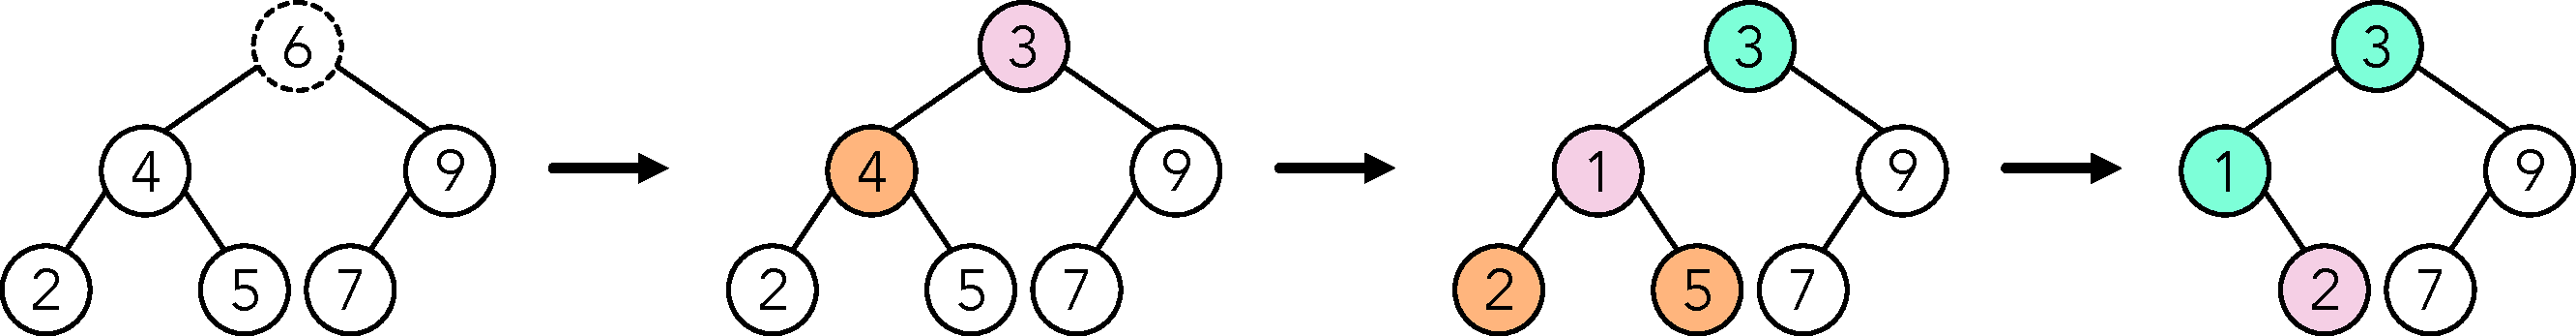
\includegraphics[width=.6\textwidth]{assets/mutate-diagram.pdf}
  \caption{Validity-preserving mutation of a binary search tree, maintaining the
  BST invariant.}\label{fig:mutation}
\end{figure}

{\em Example-Based Tuning.} Earlier we pointed out that good generators
produce ``realistic'' inputs; one way to ensure this is to tune the generator so
it produces values that are similar to some user-supplied values deemed
realistic. Existing tools make good use of this example-based approach to
tuning~\cite{soremekun2020inputs}, but they do not work with generators as
powerful as monadic generators. We implement a similar algorithm using
reflective generators: we can (1) again, reflect on the choices that lead to a
set of realistic values, and (2) run the generator with {\em new choice weights}
informed by the choices that we saw.

Both of these applications have the potential to significantly improve testing
effectiveness---example-based tuning helps users generate more realistic inputs,
adn validity-preserving mutation enables more automated approaches to improving
generator distributions---and we get {\em both} by upgrading our existing
generators to reflective ones. Additionally, we are confident that there are
more use-cases for reflective generators, which we discuss more in the following
sections.

\subsubsection{Proposed Work: Bringing Fuzzing into Focus}
{\em Fuzzers} like AFL~\cite{afl-readme} use principles that are similar to the
ones behind PBT: they both leverage randomized testing to quickly exercise as
many program behaviors as possible.  One might then expect that the fuzzing and
PBT share a significant amount of literature, but in reality they do not. Often
the communities seem to ``talk past'' one another.

We propose that the main thing separating the PBT and fuzzing communities is
simply a difference of {\em focus}. The fuzzing literature mostly talks about
fast and automatic ways to find critical (security) vulnerabilities in
programs---usually manifesting in the form of crash failures.  In contrast, PBT
researchers want effective ways to test semi-formal logical specifications of
their programs. Both areas of focus are important: fuzzing captures the ``80\%''
of cases catching high-profile bugs with minimal programmer effort, and PBT
gives a level of thoroughness that fuzzing does not claim to match. But there is
something unsatisfying when things are laid out this way. In particular, while
fuzzing and PBT focus on different testing problems, they face many of the same
technological hurdles. Both PBT and fuzzing need fast and effective ways to
generate random inputs that are valid for the systems that they are testing, and
neither community has truly settled on the ``right'' way to get there.

There is certainly some work that attempts to bridge the gap between PBT and
fuzzing. For example, FuzzChick library in Coq~\cite{OLDlampropoulos19fuzzchick}
uses code coverage as guidance for PBT and the HypoFuzz library uses a
similar approach in Python~\cite{hatfield-dodds_hypofuzz_nodate}. These projects
are demonstrably powerful, but neither benefits from the years of expertise
poured into actual fuzzers; Crowbar does~\cite{dolan2017testing}. Crowbar uses
AFL~\cite{afl-readme}, one of the most well-established
fuzzers, to generate random bit-strings that are later parsed into program
inputs.  (We plan to use AFL++~\cite{fioraldi_afl_2020},
which has supplanted the original AFL we project.)

\begin{wrapfigure}{l}{0.5\textwidth}
  \centering
  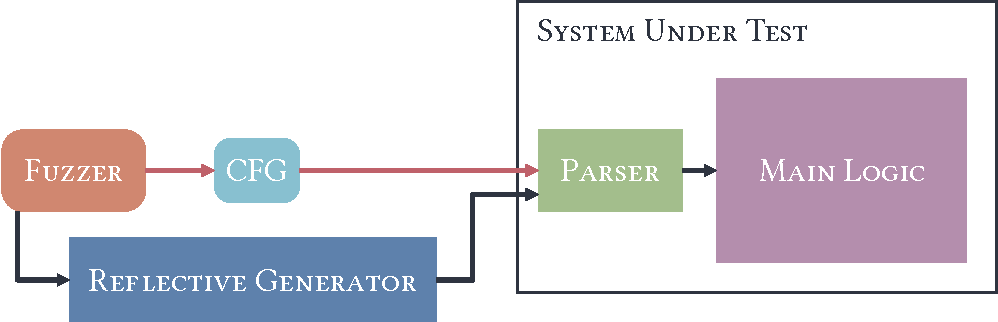
\includegraphics[width=.4\textwidth]{assets/fuzzing.pdf}
  \caption{Overview of gradually constrained fuzzing.}\label{fig:fuzzing-plan}
\end{wrapfigure}

Our system will start with a setup similar to Crowbar, but with a much greater
focus on the generators; in particular, we will use reflective generators to
gain significant testing power. The setup is shown in
Figure~\ref{fig:fuzzing-plan}. We start with a classic fuzzing setup, attempting
to make the system under test crash by passing it a variety of semi-random
inputs. Normally, the fuzzer is working against the parser, in the sense that
the parser's job is to reject invalid inputs and the fuzzer's job is to ``get
past the parser.'' The CFGs used by grammar-based fuzzers help a bit, but they
cannot generate inputs satisfying complex context-sensitive constraints. As in
Crowbar, we avoid this adversarial relationship and subsume grammar-based
generation with a powerful generator that is powerful enough to satisfy the
parser by construction; in our case, that generator is reflective.

Why use a reflective generator? First, we should clarify why any kind of monadic
generator is preferable to grammar-based options. Monadic generators can
straightforwardly generate context-free structures, and they can often do so
automatically with the help of type information~\cite{mista2019deriving}. If
this is all that the precondition requires, then there is no harm in using a
monadic generator, rather than a grammar-based one. But the beauty of a monadic
generator is that it can be made far more powerful, incrementally, as the
developer's testing needs change. The developer can start off thinking that they
need only consider the structure of their inputs, but they can later add more
semantic guarantees if they determine that their testing is ineffective.

Focusing on reflective generators specifically, one compelling benefit is that
their backward interpretation can be used to help seed the fuzzer.  Most fuzzers
ask for a number of {\em seeds}, input examples that the fuzzer can start from,
in order to ensure that the fuzzer does not spend ages exploring
inputs that have no hope of working out. Normally these seeds are easy enough
for the user to write down, since they are simply program inputs, but now that
we are asking the fuzzer to generate sequences of choices it becomes much more
error-prone (and tedious) to produce seeds by hand.  This is one great use for a
backward interpretation. The user can write down their seeds---either as values
in the program, or as text that can be parsed by the program's parser---and then
the reflective generator can reflect on the choices that produce those seeds.

The reflective generator also provides validity-preserving mutation. Guided by
heuristics, the system can opt to supplement the fuzzer's mutation schedule with
mutations that are obtained by the reflective generator's validity-preserving
mutation (which is more targeted than the mutators provided by the fuzzer). We
expect this to have a significant impact on performance, especially in contexts
where preconditions are relatively sparse and therefore hard for AFL++ to mutate
correctly.

Our ultimate goal is a grand unification of PBT and fuzzing generator tooling:
the fuzzing literature provides battle-tested heuristics for coverage-guided
generation, the PBT literature provides powerful tools like reflective
generators for refining generator performance incrementally, and both
communities benefit from generators with better distributions.

\subsubsection{Proposed Work: Reflective Shrinking}
A more modest application of reflective generators uses them to implement
validity-preserving {\em shrinking} of values to find smaller counterexamples
and speed up debugging. On its face, this feels similar to validity-preserving
mutation: Can we reflect on choices, shrink the choices, and then re-run the
generator with the smaller choices? Likely yes! But there are complications.
When mutating, it is often fine if the mutated value is accidentally quite
different from the original value, since the mutator is trying many values and
any that catch a bug are equally good. But when shrinking, it is often very
important to get another input that is both smaller and, ideally, provokes the
{\em same bug}. These nice properties are likely within reach, but care will
need to be taken to ensure that shrinkers behave as expected.

\subsection{Step 3, Validation: Understanding Testing Effectiveness \pagebudget{3}}\label{sec:val}
\subsubsection{Ongoing Work: Empirically Evaluating PBT Tools}
The many papers in the PBT literature demonstrate effectiveness with case
studies, showing that certain bugs in certain systems are caught more quickly
with one too over another. For theoretical advances, this is often sufficient
to demonstrate that the paper is worth publishing, but this kind of evaluation
can be hard to interpret from the perspective of a would-be user. \todo{Sentence
bridging to Jessica's paragraphs, linking in a theme from the intro}

\hg{Jessica is going to write us a couple of paragraphs for this}

\subsubsection{Proposed Work: Visualizing and Tuning Generator Distributions}
\newcommand{\genvis}{GenVis}
The work in Section~\ref{sec:gen} will significantly improve the tools that
users have at their disposal when designing and using random generators, but
reflective generators do not solve all of the problems developers may run into
when writing generators. One common challenge is understanding when a random
generator successfully produces an interesting distribution of values. Many
participants in our study complained that they did not really know what their
generators were doing and asked for better tools for understanding the space of
inputs that the generator covers. Tools like this would help developers catch
mistakes that hamper their testing efforts and make it easier to quickly adapt
and tune their generators to their specific needs.

Of course, understanding generator distributions is challenging.  The values
produced by generators are often highly structured and have complex shapes
(think lists, trees, and other algebraic data types). Such values cannot simply
be plotted on a chart, and even spot-checking them visually may be hard if the
values are large.  Furthermore, writing generators is already considered by
developers to be a burden, so any tool in this space needs to be incredibly
automatic and easy to use.

\begin{wrapfigure}{r}{0.6\textwidth}
  \centering
  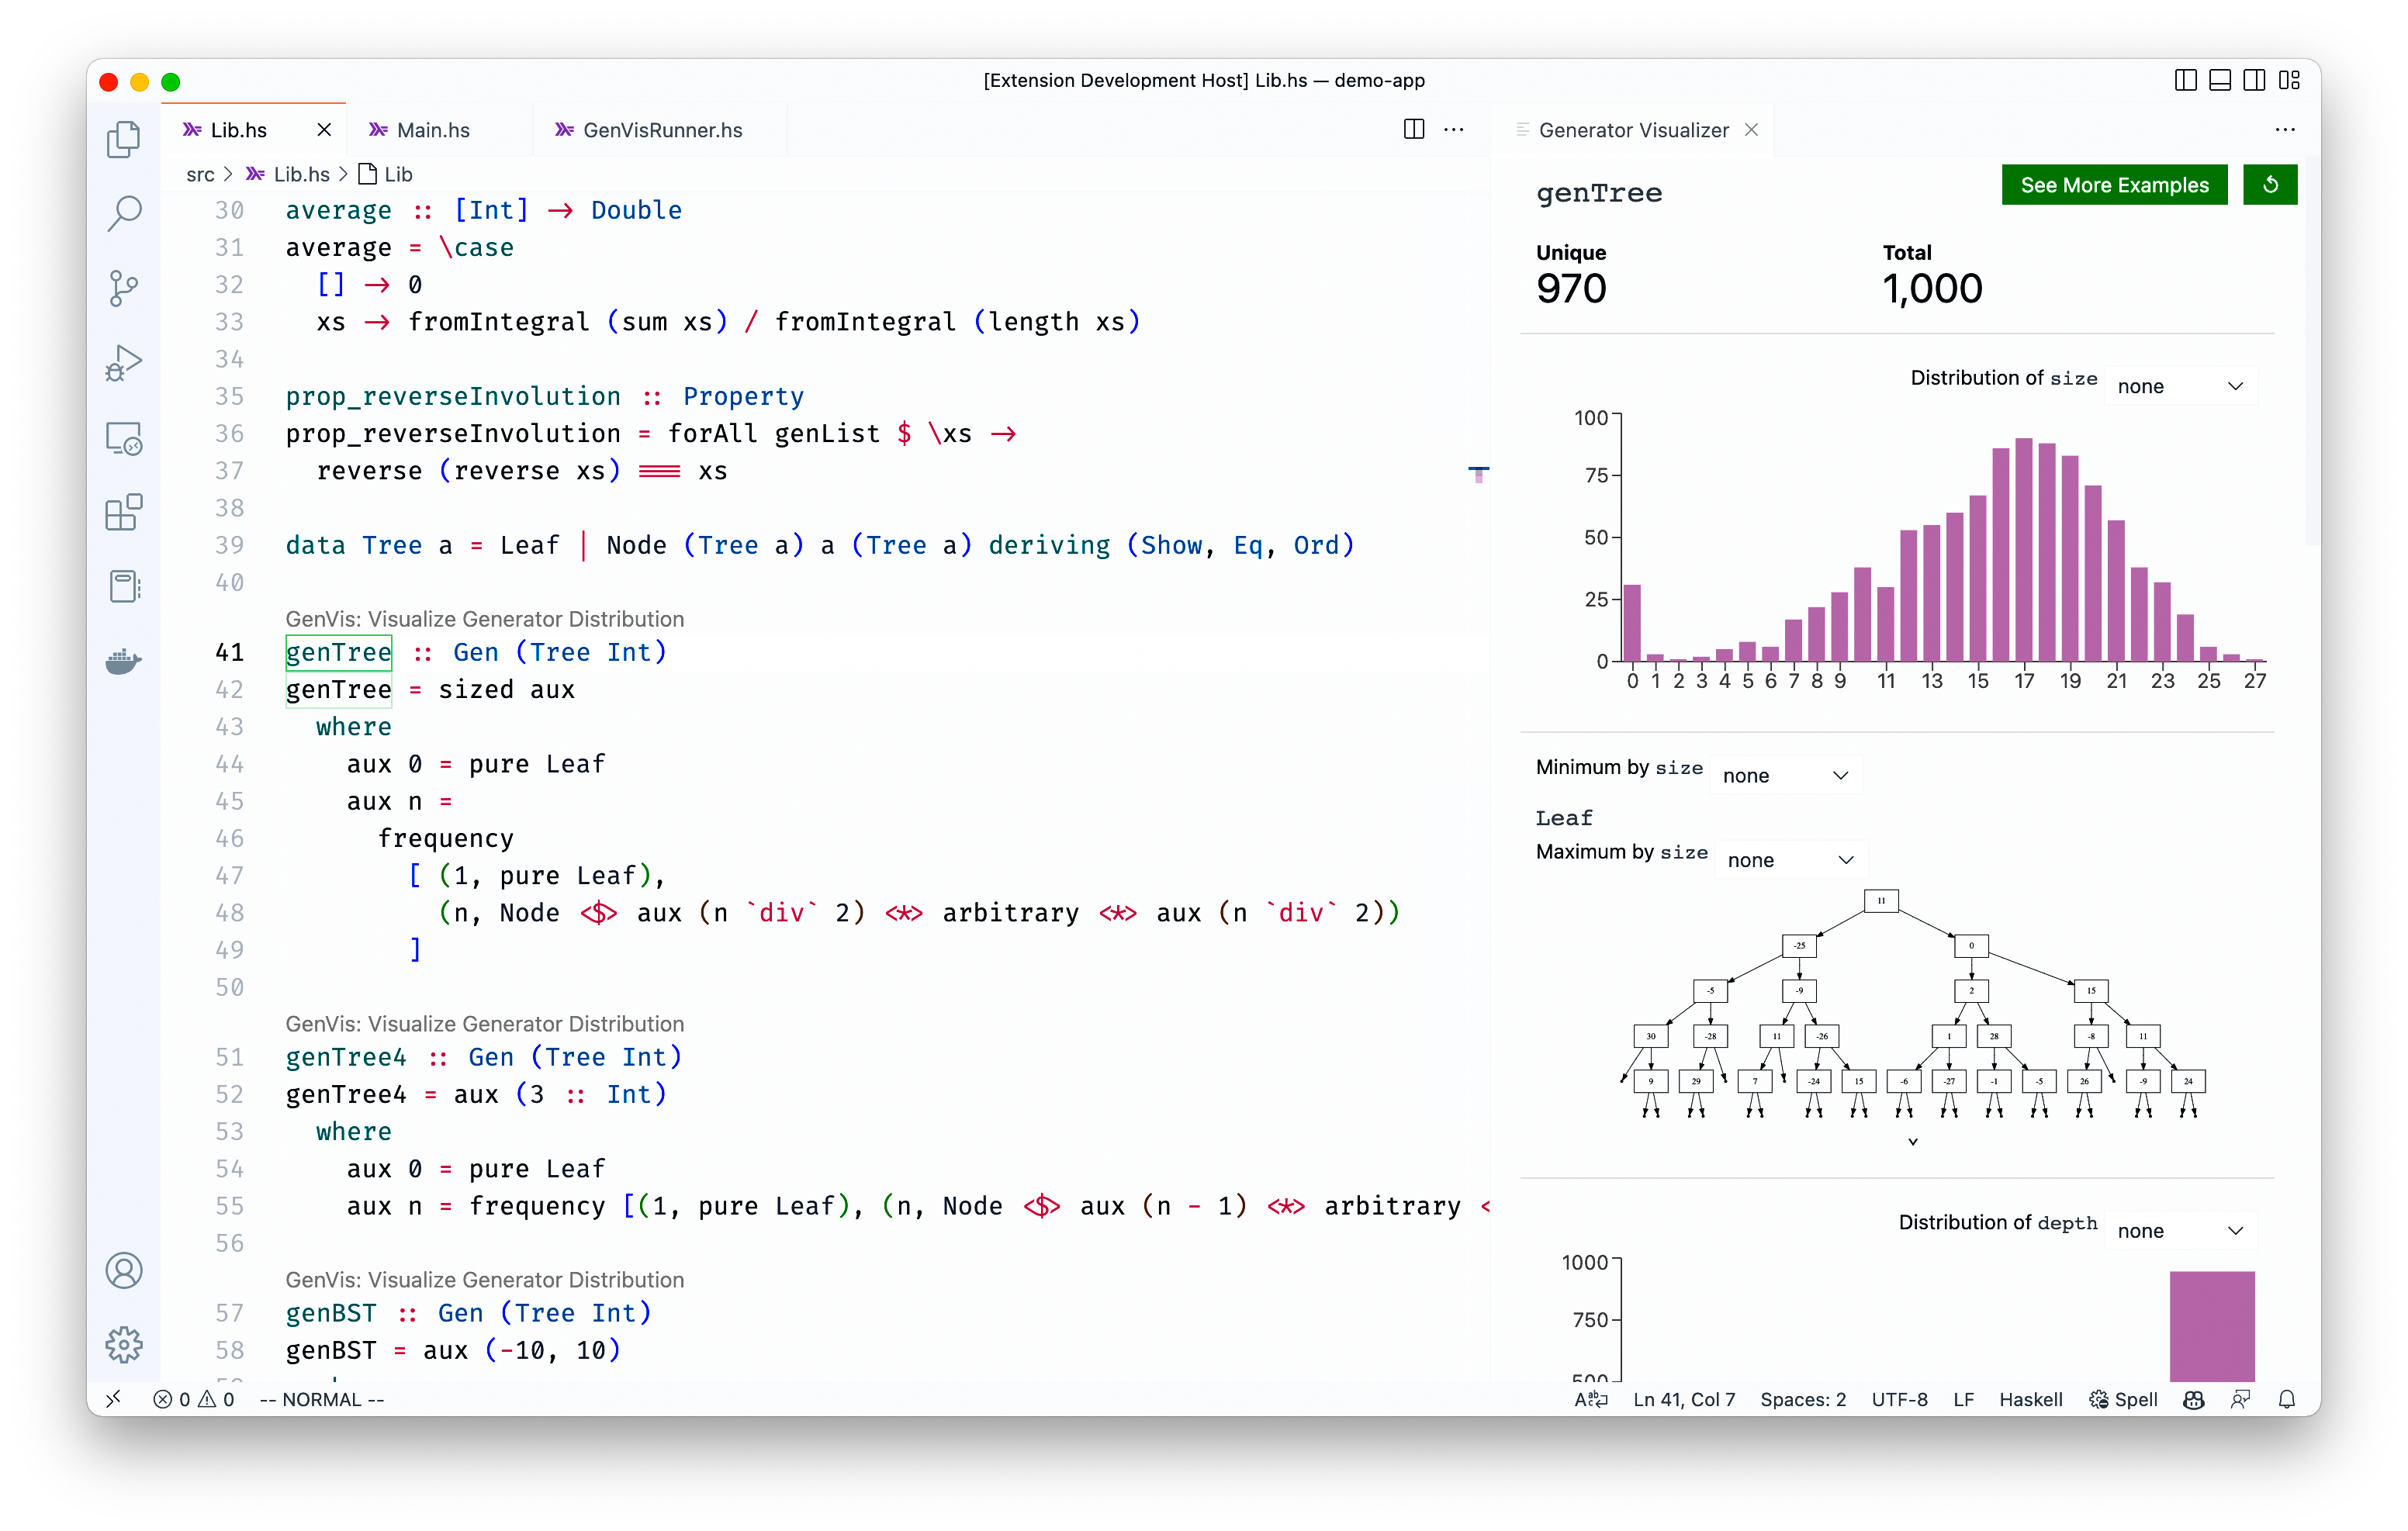
\includegraphics[width=0.6\textwidth]{assets/gen-vis.png}
  \caption{A mockup of \genvis.}\label{fig:gen-vis}
\end{wrapfigure}

With these challenges in mind, we propose prototype of \genvis, a tool that
gives developers comprehensive visualizations of their generators' distributions
from directly within their code editor. \genvis{} will address the challenges
with visualizing generator distributions by leveraging lightweight program
synthesis, visualization recommendation, and ideas from the live programming
literature.

\genvis{} starts by sampling a developer's generator and obtaining a set of
values to visualize. To get around the problem of arbitrarily structured data,
the system extracts and plots relevant {\em features} of a given datatype (e.g.,
for lists: length; for trees: size, depth, balance factor, etc.). \genvis{} will
start with a base set of features, extracted from the surrounding programming
environment and validated by the user; this will likely result in a few useful
visualizations, but maybe not enough. To ensure a comprehensive understanding of
the data, \genvis{} will then use lightweight program synthesis to compose and
combine the base of features to get {\em derived} features. The derived features
may features may show the relationship between different base features or even
compose base feature extractors to get entirely new features. All of the
features, base and derived, will be made available to users in a variety of
charts and graphs.

Of course, developers would struggle to grok dozens of charts representing
their data's features, so \genvis{} will also have a way for users to specify
which visualizations are interesting (and which to hide). We will base these
interactions based on the literature around visualization recommendation,
specifically Voyager~\cite{wongsuphasawat_voyager_2016,
wongsuphasawat_voyager_2017}. This interaction might be very quick (maybe a few
seconds to find a single representative chart) or slow and careful (many minutes
spent curating a dashboard of results to help with tuning), depending on how
much time and energy the developer has to put into their generator. Besides
charts, \genvis{} will also present the user with structured representations of
some generated values. We plan to use meta-programming to build
DOT graphs~\cite{ellson_graphviz_2002} that represent data types, and then
present those graphs to the developer for easier spot-checking of data.

All of these features will be made available to developers from within their
editor as a VSCode extension, and they will update live as the programmer edits
their generator and adds new functions that are candidates for extracting base
features. We will evaluate \genvis{} in a small user study (~15 participants),
hoping to learn which features of the tool are most useful, and how the design
may be refined into a tool that real developers can use.

\subsubsection{Proposed Work: Debugging Support for Understanding Counterexamples}

Once a PBT tool generates a counterexample of where a property fails, a
programmer will need to understand what in an input caused the program to fail.
This task can be rather challenging because generated inputs can be complex,
deep data structures \todo{Do we have a reference that implies the complexity of
generated counterexamples?}. Methods for making it clearer why a counterexample
fails could be to generate additional inputs that are very close to the
counterexample that are actually correct, to run the program up to the point
where the traces of the programs begin to diverge, and then to drop a programmer
into a debugging environment where they can query the state of the program and
step through the remainder of the execution. PI Head has prior work designing
debugging tools that help programmers understand trace divergences in an
educational setting~\cite{suzuki2017tracediff}.  \bcp{This sounds very cool!  We
should acknowledge all the work that's been done on shrinking in the PBT
community.} \amh{Good thinking!}
\hg{Hila had a similar idea that she wanted one of her undergrads to work on, we
should make sure we don't step on toes}

\subsubsection{Proposed Work: Integration with Continuous Integration Workflows}

The preliminary study suggests that one area that new developer tooling may be
needed is in managing the interplay between PBT and continuous integration (CI)
systems. Recall that developers we spoke with pointed out frustration with the
fact that PBT is both nondeterministic and long-running. This combination left
them unsure of exactly where and when to test their properties: testing
properties locally slowed down their workflow, but testing them in CI
occasionally led them to find bugs at inconvenient times.

It is likely that PBT tools could play a role in improving this state of
affairs. For example, one could take inspiration from some theorem
provers~\cite{berghofer2004random} and create a system in which properties are
checked locally but in the background, as the programmer works on other things.
This avoids waiting time while potentially being less frustrating than running
in CI, since bugs would likely be found while the programmer still had the code
``paged in.'' Alternatively, one might design a PBT system with CI in mind,
providing automated features for deferring property failure notifications until
a specified time or turning failing properties into unit tests that can be saved
for future testing.

If the full-scale study indicates that this would be a useful line of work, we
will refine these ideas via user-centered design. Rather than build a system and
hope users like it, we will build minimal prototypes and iterate on the design
by observing testers using it. Ultimately we hope this will guide us to a tool
that will meaningfully improve the experience of PBT.

\subsection{Step 4, Education: Advancing Testing in the Broader Culture \pagebudget{1}}\label{sec:ed}

\hg{This isn't actually written, this is just starter stuff from my thesis
proposal}
The preliminary study also reminded us that PBT builds on concepts that are not
always comfortable for developers, and we expect that we will learn more about
the specifics of that discomfort in the large-scale study.  Prior work has
explored ways to close this knowledge
gap~\cite{wrenn2021using,nelson2021automated}, but we expect there are further
education challenges that are worth exploring.

I hope to work with the course staff of CIS 1210 to incorporate PBT into the
curriculum. The ideal scenario would be to add a PBT thread throughout the
course, giving students the tools to specify and test their code as they go.  I
plan to follow the lead of others who have done similar things before (e.g., the
PL folks at Brown University) to give students the best chance at incorporating
PBT into their tool-set.

There are a few important challenges that need to be considered in order for
this to work out.  The curriculum is already quite full, so adding PBT likely
means removing something else. I will need to work with the professors currently
teaching the course to find room, but I expect that this process will be fairly
difficult. It is also possible that adding PBT will actually make parts of the
course {\em easier}, especially for students with some knowledge of logic and/or
less well-developed unit testing instincts. Honestly I think this is a good
thing, as it gives students more ways to succeed and it may re-enforce the value
of PBT, but some may find this problematic.

\subsection{Plan of Work \pagebudget{.7}}

\todo{(with a pretty pert chart or suchlike...)}

\subsection{Broader Impacts \pagebudget{.5}}
The Project Description must contain, as a separate section within the narrative, a section labeled ``Broader
Impacts of the Proposed Work". This section should provide a discussion of the broader impacts of the proposed
activities. Broader impacts may be accomplished through the research itself, through the activities that are
directly related to specific research projects, or through activities that are supported by, but are complementary to
the project. NSF values the advancement of scientific knowledge and activities that contribute to the
achievement of societally relevant outcomes. Such outcomes include, but are not limited to: full
participation of women, persons with disabilities, and underrepresented minorities in science, technology, engineering, and
mathematics (STEM); improved STEM education and educator development at any level; increased public
scientific literacy and public engagement with science and technology; improved well-being of individuals in
society; development of a diverse,globally competitive STEM workforce; increased partnerships between
academia, industry, and others; improved national security; increased economic competitiveness of the United
States; and enhanced infrastructure for research and education.

\subsection{Results from Prior NSF Support \pagebudget{.5}}
If any PI or co-PI identified on the project has received NSF funding (including any current
funding) in the past five years, in formation on the award(s) is required,
irrespective of whether the support was directly related to the proposal or not.
In cases where the PI or co-PI has received more than one award (excluding amendments),
they need only report on the one award most closely related to the proposal. Funding includes not just salary
support, but any funding awarded by NSF. The following information must be provided:\\

\noindent
\emph{\underline{Name of PI}}: NSF-Program (Award Number) ``Title of the Project'' (\$AMOUNT, PERIOD OF SUPPORT).
{\bf Publications:} List of publications resulting from the NSF award. A complete bibliographic citation for each
publication must be provided either in this section or in the References Cited section of the proposal); if
none, state: ``No publications were produced under this award.'' {\bf Research Products:} evidence of research products
and their availability, including, but not limited to: data, publications, samples, physical collections, software,
and models, as described in any Data Management Plan.

% \subsubsection{Proposed Study}
% The Project Description should provide a clear statement of the work to be undertaken and must include:
% objectives for the period of the proposed work and expected significance; relation to longer-term goals of the PI's
% project; and relation to the present state of knowledge in the field, to work in progress by the PI under other
% support and to work in progress elsewhere.
%
% The Project Description should outline the general plan of work, including the broad design of activities to be
% undertaken, and, where appropriate, provide a clear description of experimental methods and procedures.
% Proposers should address what they want to do, why they want to do it, how they plan to do it, how they will
% know if they succeed, and what benefits could accrue if the project is successful. The project activities may be
% based on previously established and/or innovative methods and approaches, but in either case must be well
% justified. These issues apply to both the technical aspects of the proposal and the way in which the project may
% make broader contributions.

\iflater
\subsectionstar{More stuff to not forget :-)}

Unfunded collaborations: Any substantial collaboration with
individuals not included in the budget should be described in the
Facilities, Equipment and Other Resources section of the proposal (see
Chapter II.C.2.i) and documented in a letter of collaboration from
each collaborator. Such letters should be provided in the
supplementary documentation section of FastLane or Research.gov and
follow the format instructions specified in Chapter
II.C.2.j. Collaborative activities that are identified in the budget
should follow the instructions in Chapter II.D.3.  \bcp{Jane Street.
  And maybe we should ask John too?}

bpc.net - source materials for NSF BPC plans (they also vet plans).
  we should check that other universities are doing!

\fi
